\documentclass[final]{beamer} 
\mode<presentation>
\usepackage{inconsolata}
\renewcommand*\familydefault{\ttdefault}
\usepackage{dejavu}
\renewcommand*\familydefault{\sfdefault}
\usepackage{lmodern}
\renewcommand\mathfamilydefault{\rmdefault}

\usepackage[T1]{fontenc}
\usepackage{listings}
\lstset{language=Haskell,basicstyle=\ttfamily,xleftmargin=5mm}
\usepackage{verbatim}
\usepackage{tikz}
\usetikzlibrary{arrows, fit, shapes}
\setbeamertemplate{frametitle}{
  \begin{beamercolorbox}[wd=0.95\paperwidth]{lower separation line head}
  \hspace{0.5cm}
  \insertframetitle
  \hfill
  
\includegraphics[width=.15\linewidth]{unm}
  \end{beamercolorbox}
}

\setbeamertemplate{footline}{}

\mode<all>

\definecolor{red}{RGB}{205,16,65}
\definecolor{grey}{RGB}{109,111,113}

\setbeamerfont{structure}{family=\sffamily}
\setbeamercolor{structure}{fg=red}
\setbeamerfont{normal text}{family=\sffamily}
\setbeamercolor{normal text}{fg=grey,bg=white}

\title{Subtypes for Free!}
\author{George Stelle}
\institute{University of New Mexico}
%\date{\today} 

\begin{document}
\begin{frame}[fragile]
\titlepage
\end{frame}
\begin{frame}{Types}
\centering
\onslide<1->{Why types?}
\vspace{2cm}

\onslide<2->{\emph{So evalation can't go wrong at runtime}}
\end{frame}

\begin{frame}[fragile]{Partial functions}
\onslide<1->{\texttt{head :: List a -> a}}

\onslide<2->{\texttt{tail :: List a -> List a}}

\onslide<3->{\texttt{fromJust :: Maybe a -> a}}

\onslide<4->{\texttt{bigStepEval :: Expr -> Expr}}

\onslide<5->{\texttt{warrior :: Weapon -> Warrior}}
\end{frame}

\begin{frame}[fragile]{Our Solution}
\centering
\onslide<1->{Subtypes from parametric polymorphism}

\onslide<2->{+ 

Unification}

\onslide<3->{+

Scott Encodings of ADTs}

\end{frame}

\begin{frame}[fragile]{Goal}
\onslide<1->{\texttt{head :: Cons a -> a}}

\onslide<2->{\texttt{tail :: Cons a -> List a}}

\onslide<3->{\texttt{fromJust :: Just a -> a}}

\onslide<4->{\texttt{bigStepEval :: Expr -> Value}}

\onslide<5->{\texttt{warrior :: DaggerOrSword -> Warrior}}
\end{frame}

\begin{frame}[fragile]{Subtypes from Parametric Polymorphism}

\centering
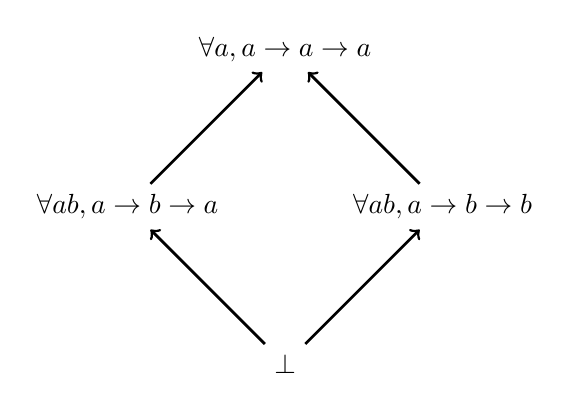
\begin{tikzpicture}[->, line width=1pt, auto, node distance=4cm]
\node (1) at (2,4) {$\forall a, a \rightarrow a \rightarrow a$};
\node (2) at (0,2) {$\forall a b, a \rightarrow b \rightarrow a$};
\node (3) at (4,2) {$\forall a b, a \rightarrow b \rightarrow b$};
\node (4) at (2,0) {$\bot$};

\path (2) edge node {} (1)
      (3) edge node {} (1)
      (4) edge node {} (2)
      (4) edge node {} (3);
\end{tikzpicture}

\end{frame}


\end{document}
